\documentclass[final,3p,times,twocolumn]{elsarticle}

%% Use the option review to obtain double line spacing
%% \documentclass[preprint,review,12pt]{elsarticle}

%% Use the options 1p,twocolumn; 3p; 3p,twocolumn; 5p; or 5p,twocolumn
%% for a journal layout:
%% \documentclass[final,1p,times]{elsarticle}
%% \documentclass[final,1p,times,twocolumn]{elsarticle}
%% \documentclass[final,3p,times]{elsarticle}
%% \documentclass[final,3p,times,twocolumn]{elsarticle}
%% \documentclass[final,5p,times]{elsarticle}
%% \documentclass[final,5p,times,twocolumn]{elsarticle}

%% if you use PostScript figures in your article
%% use the graphics package for simple commands
%% \usepackage{graphics}
%% or use the graphicx package for more complicated commands
%% \usepackage{graphicx}
%% or use the epsfig package if you prefer to use the old commands
%% \usepackage{epsfig}

%% The amssymb package provides various useful mathematical symbols
\usepackage{amssymb}
%% The amsthm package provides extended theorem environments
%% \usepackage{amsthm}
%% The bm package lets you access bold symbols in math mode using the \boldsymbol command (useful to get bold greek letters).
\usepackage{bm}
%% The bbm package is contains the indicator function symbol \mathbbm{1}
\usepackage{bbm}
%% The amsmath package contains the split environment, letting you split equations into multiple lines.
%% See "https://www.sharelatex.com/learn/Aligning_equations_with_amsmath " for an explanation.
\usepackage{amsmath}
%% The lineno packages adds line numbers. Start line numbering with
%% \begin{linenumbers}, end it with \end{linenumbers}. Or switch it on
%% for the whole article with \linenumbers after \end{frontmatter}.
%% \usepackage{lineno}
%% The algorithm defines the algorithm floating environment and the algpseudocode package is useful for constructing Pseudo code.
\usepackage{algorithm}
\usepackage{algpseudocode}
%% For creating pictures
\usepackage{tikz}
%% For making algorithms float
\usepackage{float}
\newfloat{algorithm}{t}{lop}
%% For creating draft watermark
%\usepackage{draftwatermark}
%\SetWatermarkText{DRAFT}
%\SetWatermarkScale{1}

%% Declaring \argmin and \argmax operators:
\DeclareMathOperator*{\argmin}{arg\,min}
\DeclareMathOperator*{\argmax}{arg\,max}
%% Declare trace operator \Tr:
\DeclareMathOperator*{\Tr}{Tr}
%% Declare pdf functions
\DeclareMathOperator*{\Cat}{Cat}
\DeclareMathOperator*{\Dir}{Dir}
\DeclareMathOperator*{\DP}{DP}
\DeclareMathOperator*{\Beta}{Beta}
\DeclareMathOperator*{\GEM}{GEM}
\DeclareMathOperator*{\Stick}{Stick}
%% shorthand for \boldsymbol
\let\bs\boldsymbol
%% command that allows equations to be split across pages
%\allowdisplaybreaks[3]

%% natbib.sty is loaded by default. However, natbib options can be
%% provided with \biboptions{...} command. Following options are
%% valid:

%%   round  -  round parentheses are used (default)
%%   square -  square brackets are used   [option]
%%   curly  -  curly braces are used      {option}
%%   angle  -  angle brackets are used    <option>
%%   semicolon  -  multiple citations separated by semi-colon
%%   colon  - same as semicolon, an earlier confusion
%%   comma  -  separated by comma
%%   numbers-  selects numerical citations
%%   super  -  numerical citations as superscripts
%%   sort   -  sorts multiple citations according to order in ref. list
%%   sort&compress   -  like sort, but also compresses numerical citations
%%   compress - compresses without sorting
%%
%% \biboptions{comma,round}

% \biboptions{}


\journal{MPhil in Scientific Computing}

\begin{document}

\begin{frontmatter}

%% Title, authors and addresses

%% use the tnoteref command within \title for footnotes;
%% use the tnotetext command for the associated footnote;
%% use the fnref command within \author or \address for footnotes;
%% use the fntext command for the associated footnote;
%% use the corref command within \author for corresponding author footnotes;
%% use the cortext command for the associated footnote;
%% use the ead command for the email address,
%% and the form \ead[url] for the home page:
%%
%% \title{Title\tnoteref{label1}}
%% \tnotetext[label1]{}
%% \author{Name\corref{cor1}\fnref{label2}}
%% \ead{email address}
%% \ead[url]{home page}
%% \fntext[label2]{}
%% \cortext[cor1]{}
%% \address{Address\fnref{label3}}
%% \fntext[label3]{}

\title{Mini Project: Dirichlet Processes and the Dirichlet Process Mixture}

%% use optional labels to link authors explicitly to addresses:
%% \author[label1,label2]{<author name>}
%% \address[label1]{<address>}
%% \address[label2]{<address>}

\author{Brian Azizi}

\address{Cavendish Laboratory, Department of Physics, J J Thomson
  Avenue, Cambridge. CB3 0HE}

\begin{abstract}
As part of the written assignment for the MPhil in Scientific Computing, we have implemented three clustering algorithms in the C++ programming language: the k-means algorithm, the Gaussian mixture model and the Dirichlet Process mixture model.
Subsequently, the algorithms will be compared and texted on a number of data sets.
\end{abstract}

\end{frontmatter}

%%
%% Start line numbering here if you want
%%
% \linenumbers

%% main text
\section{Introduction}
\label{sect:Intro}
In this written assignment, we introduce the \emph{Dirichlet Process Mixture (DPM)} as a \emph{non-parametric Bayesian} model for clustering.
We begin with a general discussion of Dirichlet Processes (DP).
We then give four different representations of DPs that give us a deeper intuitive understanding in section \ref{sect:representations}.
Section \ref{sect:DPM} explains how Dirichlet processes can be applied to clustering via the Dirichlet Process Mixture.
Following this, we discuss inference in the DPM and our implementation of the model.
Here, we will also give some output of our implementation.
In the final section, we discuss further work and conclude.

\section{Bayesian Parametrics and the Dirichlet Distribution}
In this section, we describe the Dirichlet distribution.

\subsection{Discrete Random Variables and the Categorical Distribution}
Consider a discrete random variable $x$ that can take one of $K$ possible categorical values, $x \in \{1,\dots,K\}$.
The distribution of $x$ is then fully specified by the probabilities $\pi_k = P(x = k)$ and its probability mass function (pmf) is given by
\begin{equation}
\label{eqn:catpmf}
p(x\,|\,\pi_1,\dots,\pi_K) = \prod_{k=1}^K \pi_k^{\,\delta_{x,k}}
\end{equation}
where we made use of the Kronecker delta defined by
\begin{equation}
\label{eqn:kronecker}
\delta_{i,j} := \mathbbm{1}\{i = j\} = \left\{\begin{array}{lr}
1 & \mbox{if $i = j$}\\
0 & \mbox{otherwise} \end{array} \right.
\end{equation}

We say that $x$ follows the \emph{categorical distribution}
\footnote{This distribution is sometimes also referred to as the \emph{Discrete}, the \emph{Multinoulli} or (somewhat inaccurately) the \emph{Multinomial} distribution.}
, denoted $x \sim Cat(\pi_1, \dots, \pi_K)$.
This can be viewed as a generalization of the Bernoulli distribution to more than two outcomes.
Alternatively, we can specify the distribution of $x$ through a \emph{(generalized) probability density function (pdf)} by making use of the \emph{Dirac delta function}.
\footnote{The Dirac delta can be loosely thought of as a function on $\mathbb{R}$ which is zero everywhere except at the origin where it is infinite,
\[\delta(x) = \left\{
\begin{array}{ll}
+\infty, & x = 0\\
0, & \mbox{otherwise}
\end{array} \right.\]
and whose integral over the real line is unity
\[ \int_{-\infty}^{+\infty}\delta(x)dx = 1.\]
Note however, that this is not a formal definition. $\delta$ can be rigorously defined using measure theory or the theory of generalized functions.}

\begin{equation}
\label{eqn:catpdf}
\Cat(x\,|\,\pi_1,\dots,\pi_K) = \sum_{k=1}^K \pi_k \delta(x - k)
\end{equation}

Generalized probability density functions greatly unify the analysis of discrete and continuous random variables (as well as variables that are discrete on some parts of the probabiliy space and continuous on others).
For instance, the usual definitions of expectation, variance, etc for continuous variables can be directly carried over to the case of discrete variables.
In this context, points in probability space with non-zeros probability mass are referred to as \emph{atoms} (thus, the pdf of categorical variables consists entirely of atoms).
Figure \ref{fig:pmf} illustrates the pdf of $x$.

\begin{figure}
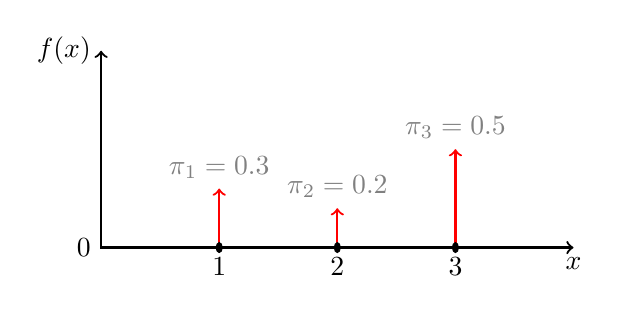
\begin{tikzpicture}[yscale=2.5,xscale=1.5]
\draw[thick,<->] (0,1)node [left] {$f(x)$} -- (0,0) node [left] {$0$} -- (4,0) node [below] {$x$};
\draw[red,thick,->] (1,0) -- (1,0.3) node [above,gray] {$\pi_1 = 0.3$};
\draw[red,thick,->] (2,0) -- (2,0.2) node [above,gray] {$\pi_2 = 0.2$};
\draw[red,thick,->] (3,0) -- (3,0.5) node [above,gray] {$\pi_3 = 0.5$};
\draw[fill] (1,0) circle [radius=0.025] node [below] {$1$};
\draw[fill] (2,0) circle [radius=0.025] node [below] {$2$};
\draw[fill] (3,0) circle [radius=0.025] node [below] {$3$};
\end{tikzpicture}
\caption{The probability density function of a discrete random variable that can occupy 3 possible states, $f(x) = \Cat(x\,|\,\pi_1,\pi_2,\pi_3)$.}
\label{fig:pmf}
\end{figure}

In order for the pmf and the pdf of the categorical distribution to be well-defined, we require that $\pi_k \geq 0$ and $\sum_{k=1}^K \pi_k = 1$ since the $\pi_k$ represent probabilities.
In other words, we require $\bs \pi = (\pi_1,\dots,\pi_K)$ to live on the \emph{$K$-dimensional probability simplex}
\footnote{Note however that, due to the sum-to-one constraint, $\Delta_K$ is in fact only a $(K-1)$-dimensional manifold embedded in $K$-dimensional Euclidean space.
For this reason, some authors refer to $\Delta_K$ as the $(K-1)$-dimensional probability simplex (and use the notation $\Delta_{K-1}$ instead).}
defined as
\begin{equation}
\label{eqn:simplex}
\Delta_K = \left\{(\pi_1,\dots,\pi_K) \in \mathbb{R}^K : \pi_k \geq 0,\,\, \sum \nolimits _{k=1}^K \pi_k = 1\right\}.
\end{equation}
Figure \ref{fig:simplex} depicts $\Delta_K$ when $K=3$.

\begin{figure}
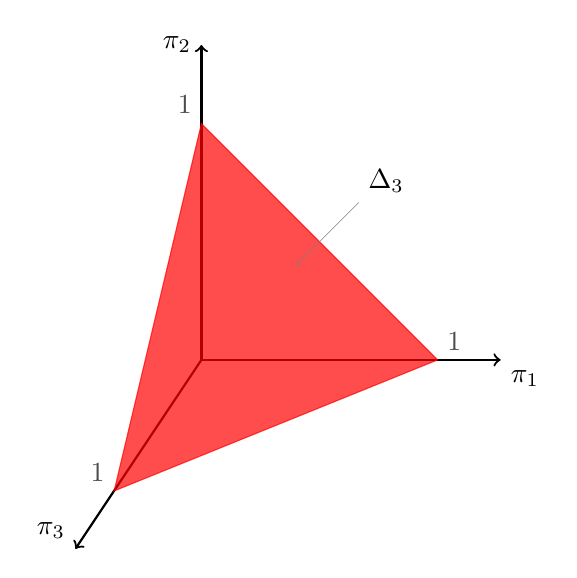
\begin{tikzpicture}[scale=2]
\draw[thick,<-] (0,2) node [left] {$\pi_2$} -- (0,0);
\draw[thick,->] (0,0) -- (1.9,0) node [below right] {$\pi_1$};
\draw[thick,->] (0,0) -- (-0.8,-1.2) node [above left] {$\pi_3$};
\draw[red, fill=red, opacity=0.7] (1.5,0) node [above right, black] {$1$} -- (0,1.5) node [above left, black] {$1$} -- (-.554,-.832) node [above left, black] {$1$} -- (1.5,0);
\draw[help lines,<-] (0.6,0.6) -- (1,1) node [above right, black] {$\Delta_3$};
\end{tikzpicture}
\caption{The 3-dimensional probability simplex $\Delta_3$.}
\label{fig:simplex}
\end{figure}

Now suppose we have a dataset $S=\{x_{(i)}\}_{i=1}^N$ consisting of $N$ independent observations of $x$.
The corresponding likelihood function takes the form
\begin{equation}
\label{eqn:catlik}
\begin{split}
p(S\,|\,\bs \pi) &= \prod_{i=1}^N \prod_{k=1}^K \pi_k^{\delta_{x^{(i)},k}} \\ &= \prod_{k=1}^K \pi_k^{\left(\sum_{i=1}^N \delta_{x^{(i)},k}\right)} = \prod_{k=1}^K \pi_k^{\,m_k}
\end{split}
\end{equation}
where $m_k = \sum_{i=1}^N \delta_{x^{(i)}, k}$ represents the number of observation in which $x$ takes the value $k$.
The quantities $m_k$ are the sufficient statistics of the categorical distribution.

\subsubsection*{\normalfont \small \bfseries Maximum Likelihood Inference}
In the frequentist setting, we typically infer the parameter $\bs \pi$ through maximum likelihood estimation.
Given dataset $S$, we choose $\bs \pi$ that maximises the log of the likelihood function $p(S\,|\,\bs \pi)$ taking into account the constraint that $\bs \pi \in \Delta_K$.
To perform the constrained optimization, we use the method of Lagrange multipliers. We form the Lagrangian
\footnote{Generally speaking, we should include the inequality constraints $\pi_k \geq 0$ in the Lagrangian and perform the optimization via the Karush-Kuhn-Tucker conditions.
In our case we may safely ignore these constraints since our solution (equation \ref{eqn:catML}) happens to satisfy them regardless.}
using equation \ref{eqn:catlik}

\begin{equation}
\label{eqn:catlagrange}
\begin{split}
L(\bs \pi, \lambda) &= \log p(S\,|\,\bs \pi) + \lambda\left(1 - \sum \nolimits_{k=1}^K \pi_k\right)\\
&= \sum\nolimits_{k=1}^K m_k \log \pi_k + \lambda\left(1-\sum\nolimits_{k=1}^K \pi_k\right)
\end{split}
\end{equation}

Setting the derivate of $L$ with respect to the Lagrange multiplier $\lambda$ to zero, we get our sum-to-one constraint
\begin{equation}
\label{dldlambda}
\frac{\partial L}{\partial \lambda} = 1 - \sum\nolimits_{k=1}^K = 0.
\end{equation}
Differentiating with respect to $\pi_k$ gives
\begin{equation}
\frac{\partial L}{\partial \pi_k} = \frac{m_k}{\pi_k} - \lambda
\end{equation}
and setting the derivative to zero yields

\begin{equation}
\label{dldpi}
\begin{split}
\lambda \pi_k &= m_k\\
\Rightarrow \lambda \sum\nolimits_k \pi_k &= \sum\nolimits_k m_k\\
\Rightarrow \lambda &= N
\end{split}
\end{equation}

Therefore, the maximum likelihood solution is 
\begin{equation}
\label{eqn:catML}
\pi_k = \frac{m_k}{N}
\end{equation}
which is simply the fraction of observations in which $x = k$.

\subsection{The Dirichlet Distribution and Bayesian Inference}
\label{sect:dirdistro}
\begin{figure*}
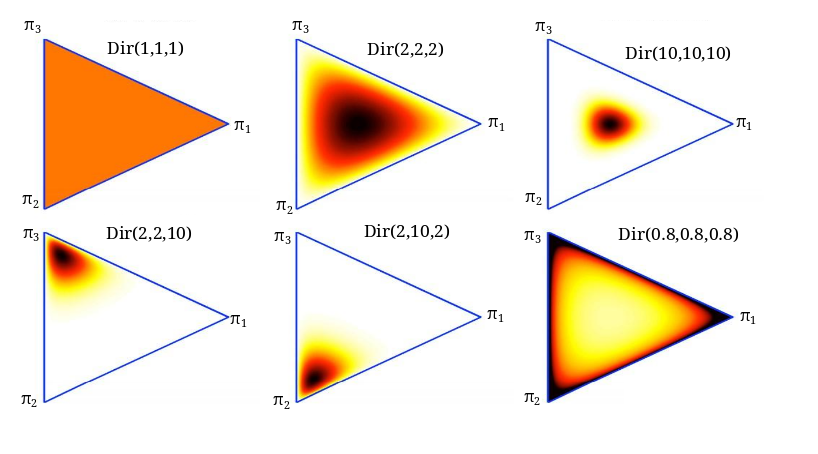
\includegraphics[width=\textwidth,height=4in]{dir.png}
\caption{Examples of Dirichlet distributions on $\Delta_3$. (Figure from \cite{ywt07})}
\label{fig:dir}
\end{figure*}

If our dataset is small (e.g. $N < K$), the maximum likelihood approach might (incorrectly) estimate many of the parameters to be zero.
Based on this analysis, we would conclude that the probability of a new sample $x^{(N+1)}$ taking on certain values to be zero.
This is sometimes referred to as the \emph{zero count problem}.

In this section, we give a quick discussion on Bayesian inference for our categorical variable $x$. Along the way, we will introduce the Dirichlet distribution and demonstrate how the Bayesian framework is less prone to the zero count problem.

In a Bayesian framework, we need to specify a prior distribution $p(\bs \pi)$for our model parameters $\bs \pi$. We then use our dataset $S$ to update the prior and obtain a posterior distribution $p(\bs \pi\,|\,S)$ for $\bs \pi$.
The update is done in accordance with Bayes rule
\begin{equation}
\label{eqn:bayes}
p(\bs \pi \,|\, S) = \frac{p(S\,|\,\bs \pi) p(\bs \pi)}{\int_{\bs \pi} p(S\,|\,\bs \pi)p(\bs \pi)d\bs\pi}.
\end{equation}
In general, the integral in the denominator is analytically intractable and numerical approximations can be very computationally intensive.
However, for some likelihood models, we can find a parametric family of distributions such that the prior and the posterior are both members of that family. 
The prior is then said to be \emph{conjugate} to the likelihood function and the parameters of the conjugate family are referred to as \emph{hyper-parameters}.
If we have conjugacy, computing the posterior is simply a matter of updating the hyper-parameters.

\subsubsection*{\normalfont \small \bfseries Dirichlet Distributions}
Looking at equation \ref{eqn:catlik} we see that the conjugate prior to a categorical likelihood function needs to have support over the probability simplex $\Delta_K$ and have a pdf of the form 
\begin{equation}
p(\bs \pi) \propto \prod\nolimits_{k=1}^K \pi_k^{\hat\alpha_k}.
\end{equation}
The Dirichlet distribution satisfies both criteria. 
It has support over the probability simplex $\Delta_K$ and its pdf
\footnote{
$\Gamma(t)$ is the \emph{Gamma function} defined as 
\[
\Gamma(t) = \int\nolimits_{-\infty}^{\infty} x^{t-1} e^{-x} dx
\]	
for $t \in \mathbb{R}_+$.
It is a generalization of the factorial function to the positive real line since for $n\in \mathbb{N}$, $\Gamma(n) = (n-1)!$.
}
is defined as
\begin{equation}
\label{eqn:dirpdf}
\Dir(\bs \pi\,|\,\bs \alpha) = \mathbbm{1}\{\bs \pi \in \Delta_K\}\frac{\Gamma(\sum_{k=1}^K\alpha_k)}{\prod_{k=1}^K\Gamma(\alpha_k)}\prod\nolimits_{k=1}^K\pi_k^{\alpha_k - 1} 
\end{equation}
The quantities $(\alpha_1,\dots,\alpha_K)$ are the \emph{concentration parameters} of the distribution and we require them to be strictly positive real numbers. 
Figure \ref{fig:dir} shows heat plots of the dirichlet pdf over $\Delta_3$ for different parameter values $\bs \alpha$.
When $\alpha_k = 1$ for all values of $k$ we get the uniform distribution.
If $\alpha_k  > 1$ we get a unimodal distribution where the position of the peak depends on the relative sizes of the $\alpha_k$ and the size of the peak depends on the magnitudes of the $\alpha_k$.
For $\alpha_k < 0$, the distribution is unbounded, multimodal and the probability mass concentrates on the edge of the simplex.

Define $\alpha_0 = \sum_{k=1}^K \alpha_k$. To work out the mean of a Dirichlet distributed variable, we first find the mean of the first component $\pi_1$,
\begin{equation}
\label{eqn:dirmean1}
\begin{split}
\mathbbm{E}\left[\pi_1\right] &= \frac{\Gamma(\alpha_0)}{\prod_{k=1}^K\Gamma(\alpha_k)} \int\nolimits_{S_K} \pi_1 \Dir(\bs \pi \,|\, \bs \alpha)d\bs\pi \\
&= \frac{\Gamma(\alpha_0)}{\prod_{k=1}^K\Gamma{\alpha_k}} \left[\int_0^1\int_0^{1-\pi_1}\dots\int_0^{1-\sum_{k=1}^{K-1}} \right.\\
& \left.\pi_1^{\alpha_1}\pi_2^{\alpha_2-1}\dots\pi_K^{\alpha_K-1}d\alpha_K \dots d\alpha_1\right]\\
&= \frac{\Gamma(\alpha_0)}{\prod_{k=1}^K\Gamma(\alpha_k)} \frac{\Gamma(\alpha_1+1)\prod_{k=2}^K\Gamma(\alpha_k)}{\Gamma(\alpha_0+1)}\\
&= \frac{\Gamma(\alpha_0)}{\prod_{k=1}^K\Gamma(\alpha_k)} \frac{\alpha_1\prod_{k=1}^K\Gamma(\alpha_k)}{\alpha_0 \Gamma(\alpha_0)}\\
&= \frac{\alpha_1}{\alpha_0}
\end{split}
\end{equation}
where we used the fact that the integral is the normalization constant of the $\Dir(\alpha_1+1,\alpha_2,\dots,\alpha_K)$ pdf in the third line and the property of the Gamma function that $\Gamma(t+1)=t\Gamma(t)$ in the fourth line. 
The derivation is symmetric for the remaining components of $\bs \pi$, thus 
\begin{equation}
\label{eqn:dirmean}
\mathbbm{E}\left[\bs \pi \right] = \frac{\bs \alpha}{\alpha_0}
\end{equation}

Often, a symmetric Dirichlet distribution of the form $\alpha_k = \alpha \forall k$ is used as prior.
In this case, the mean of the $k$th component of $\pi_k$ is $\mathbbm{E}\left[\pi_k\right] = 1/K$.
It can be shown that the variance of $\pi_k$ is given by
\begin{equation}
\label{eqn:dirvar}
\mathbb{V}\left[\pi_k\right] = \frac{K-1}{K^2(\alpha K + 1)}.
\end{equation}
In this case, $\alpha$ corresponds to the inverse variance of the distribution.

\subsubsection*{\normalfont \small \bfseries Conjugate Bayesian Inference of Categorical Variables}
Previously, we had $x\,|\,\bs \pi \sim Cat(\pi_1,\dots,\pi_K)$.
Suppose we give $\bs \pi$ a Dirichlet prior: $\bs \pi \sim \Dir(\bs \alpha)$.

Once we have a set of observations $S = \{x^{(i)}\}_{i=1}^N$, we are interested in how this affects our believe about the parameters $\bs \pi$, i.e. what is the posterior?
From equation \ref{eqn:bayes}, we know that the posterior pdf, $p(\bs \pi \,|\, S)$ of $\bs \pi$ is proportional to the likelihood function $p(S\,|\,\bs \pi)$ times the prior pdf $p(\bs \pi)$.
Thus, from equations \ref{eqn:catlik} and \ref{eqn:dirpdf}, we get
\begin{equation}
\label{eqn:dirpost}
\begin{split}
p(\bs \pi \,|\, S) &\propto \prod\nolimits_{k=1}^K\pi_k^{m_k} \prod\nolimits_{k=1}^K \pi_k^{\alpha_k - 1}\\
	&= \prod\nolimits_{k=1}^K \pi_k^{\alpha_k+m_k-1}
\end{split}
\end{equation}
and we recognize this as the pdf of a Dirichlet distribution with parameter vector $(\alpha_1+m_1,\dots,\alpha_K+m_K) = \bs \alpha + \bs m$.

The \emph{posterior predictive distribution} of our model (that is, the distribution that a new sample $x^{(N+1)}$ would have, conditional on the observed data $S$) is obtained by marginalising out the model parameters $\bs \pi$ over the posterior distribution:
\begin{equation}
\begin{split}
p(X = k\,|\,S, \bs \alpha) &= \int p(X = k\,|\,\bs \pi)p(\bs \pi \,|\,S)d\bs\pi\\
&= \int p(X = k\,|\,\pi_k)\left[\int p(\bs \pi_{-k},\pi_k\,|\,S)d\bs\pi_{-k}\right]d\pi_k\\
&= \int \pi_k p(\pi_k\,|\,S)d\pi_k\\
&= \mathbb{E}\left[\pi_k\,|\,S\right]\\
&= \frac{\alpha_k + m_k}{\sum_j (\alpha_j+m_j)} = \frac{\alpha_k+m_k}{\alpha_0 + N}
\end{split}
\end{equation}
where we use $\bs \pi_{-k}$ to denote all components of $\bs \pi$ except $\pi_k$.

Note that this method of prediction circumvents the zero count problem.
We also see that we may interpret the hyperparameters as \emph{pseudo data}.
$\alpha_0$ is the effective size of the pseudo data set and $\alpha_k$ is the effective number of times that $x$ takes on value $k$ in the pseudo data.
The posterior distribution of $\bs \pi$ takes into account both our prior believe about $x$ (via the pseudo data) and the actual observed data.

For future reference, we also state the \emph{prior predictive distribution} of our model.
This is the distribution of a sample $X$ before any data is observed and is obtained by marginalising out $\bs \pi$ over its prior:
\begin{equation}
\label{eqn:dirpriorpredictive}
p(x = k\,|\,\bs \alpha) = \frac{\alpha_k}{\alpha_0}
\end{equation}
which is just the prior expected value of $\pi_k$.
Thus, $x \sim \Cat(\frac{\alpha_1}{\alpha_0},\dots,\frac{\alpha_K}{\alpha_0})$.

For more information on the Bayesian and frequentist analysis of categorical data and the Dirichlet distribution, see \cite{Bishop, Murphy}.
\section{The Dirichlet Process}
\label{sect:dp}
Having discussed the Dirichlet distribution and its role in the parametric Bayesian analysis of discrete random variables, we are now ready to explore the Dirichlet process and its role in Bayesian nonparametrics.
In this section, we will first give an informal description of the Dirichlet process and show how draws from a Dirichlet process can be visualized.
We then give a formal mathematical definition of the DP and discribe its parameters.

\subsubsection*{\normalfont \small \bfseries From the Dirichlet Distribution to the Dirichlet Process}
We saw that the Dirichlet distribution can be used as a prior for categorical variables when the number of possible states $K$ is finite and known. Draws from a Dirichlet distribution give us a probability vector $\bs \pi$ of length $K$. For this reason, we can think of the Dirichlet distribution as a distribution over distributions.

The Dirichlet Process is the non-parametric extension of the Dirichlet distribution.
Instead of a random vector $\bs \pi$, a draw from a Dirichlet process is a \emph{random function} $G$ with certain properties.
And analogously to $\bs \pi$ being a valid probability distribution (since $\bs \pi$ lives on the probability simplex $\Delta_K$), $G$ is a valid probability function, a so-called \emph{probability measure}.
A probability measure is a (set) function that maps subsets from some probability space $\Omega$ onto the unit interval $[0,1]$ and that satisfies certain properties.
The most notable properties are that $G(\emptyset)=0$, $G(\Omega)=1$ and if $A_1,A_2,\dots$ are pairwise disjoint subsets of $\Omega$ (meaning $A_i\cap A_j = \emptyset$ if $i\neq j$), then $G(\cup_{i=1}^\infty A_i) = \sum_{i=1}^\infty G(A_i)$.
\footnote{There are also conditions on the domain of a measure.
The collection of subsets of $\Omega$ on which a measure is defined is called a \emph{$\sigma$-algebra} of $\Omega$.
A $\sigma$-algebra must contain the empty subset, be closed under complement and be closed under union or intersection of countably many subsets.}

In the parametric case, our categorical variable $x$ could take on an integer between $1$ and $K$.
Thus, our probability space in that case was $\Omega = \{1,\dots,K\}$.
In equation \ref{eqn:catpdf} we defined a probability density for $x$.
It is also possible to define a probability measure $\mu$ on $A \subset \Omega$ using the \emph{Dirac measure} defined by
\footnote{This is the third $\delta$-type object we have introduced in this document.
Both the Kronecker delta and the Dirac delta function can be thought of as special cases of the Dirac measure.}
\begin{equation}
\label{eqn:diracmeasure}
\delta_x(A) = \left\{ \begin{array}{lr}
1 & \mbox{if $x \in A$} \\
0 & \mbox{otherwise}
\end{array} \right.
\end{equation}
The measure $\mu$ can then be expressed as 
\begin{equation}
\label{eqn:discretemeasure}
\mu(A) = \sum\nolimits_{k=1}^K \pi_k \delta_x (A)
\end{equation}
and is known as the \emph{discrete measure}. 

In the case of the Dirichlet process, the $\Omega$ can be any general valid probability space (not necessarily finite or even countable) and $G$ can be any probability measure on $\Omega$.
If we have a random variable $\theta$ that takes values in $\Omega$, then the measure $G$ induces a probability distribution for $\theta$.
If $A$ is measurable subset of $\Omega$, we can define $Pr(\theta \in A) = G(A)$.
%However, it turns out that draws from a Dirichlet process are discrete measures on $\Omega$ almost surely (i.e. with probability one).

\subsubsection*{\normalfont \small \bfseries A mathematical definition of the Dirichlet process}
Let $A_1,\dots,A_K$ be a finite partition of $\Omega$.
This means $A_1 \cup \dots \cup A_K = \Omega$ and $A_k$ are pairwise disjoint.
If $G$ is a measure on $\Omega$, then $(A_k)$ is some number between $0$ and $1$ and $\sum_{k=1}^K G(A_k) = 1$.
In other words, the vector $G(A_1),\dots,G(A_K)$ lives on the probabilty simplex $\Delta_K$.
Suppose now that $G$ is randomly drawn from a Dirichlet process, $G \sim \DP$.
Then $(G(A_1),\dots,G(A_K))$ is a random vector and we can specify a distribution for it.

\begin{figure}
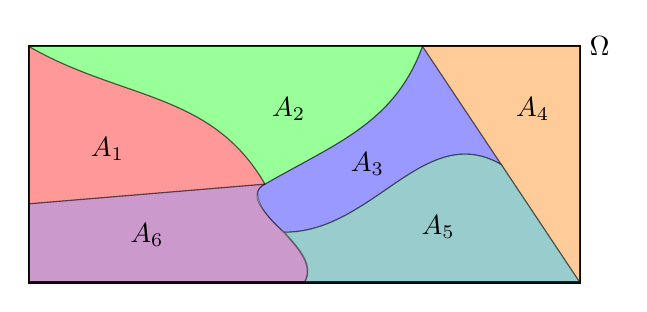
\begin{tikzpicture}[scale=1]
\draw [thick] (0,0) rectangle (7,3);
\draw [fill=red,opacity=0.4] (0,3) to [out=330, in=120] (3,1.25) to (0,1) to (0,3);
\node at (1,1.7) {$A_1$};
\draw [fill=green,opacity=0.4] (0,3) to [out=330, in=120] (3,1.25) to [out=30,in=250] (5,3);
\node at (3.3,2.2) {$A_2$};
\draw [fill=blue,opacity=0.4] (3,1.25) to [out=30,in=250] (5,3) to (6,1.5) to [out=150,in=0] (3.25,0.64) to [out=145,in=200] (3,1.25);
\node at (4.3,1.5) {$A_3$};
\draw [fill=orange,opacity=0.4] (5,3) -- (7,0) -- (7,3) -- (5,3);
\node at (6.4,2.2) {$A_4$};
\draw [fill=teal,opacity=0.4] (7,0) to (6,1.5) to [out=150,in=0] (3.25,0.64) to [out=310,in=60] (3.5,0) to (7,0);
\node at (5.2,0.7) {$A_5$};
\draw [fill=violet,opacity=0.4] (3,1.25) to [out=210,in=60] (3.5,0) to (0,0) to (0,1) to (3,1.25);
\node at (1.5,0.6) {$A_6$};
\node at (7,3) [right] {$\Omega$};
\end{tikzpicture}
\caption{A finite partition of $\Omega$.}
\label{fig:partition}
\end{figure}

The Dirichlet process is implicitly defined by the requirement that $(G(A_1), \dots, G(A_K))$ has a joint Dirichlet distribution.
We write 
\[G \sim \DP(\alpha,H)\]
if 
\begin{equation}
\label{eqn:dpdef}
(G(A_1),\dots,G(A_K)) \sim \Dir(\alpha H(A_1), \dots, \alpha H(A_K))
\end{equation}
for any finite partition $A_1,\dots,A_K$ of $\Omega$.

A Dirichlet process is specified by a \emph{concentration parameter} $\alpha$ which is a positive real number, and a \emph{base measure} $H$ which is a probability measure on the probability space $\Omega$.
Two describe the expectation and variance of Dirichlet process distributed measure $G$, consider any measurable subset $A$ of $\Omega$. 
The expectation is given by
\begin{equation}
\label{eqn:meandp}
\mathbb{E}\left[G(A)\right] = H(A)
\end{equation}
and the variance is given by
\begin{equation}
\label{eqn:vardp}
\mathbb{V}\left[G(A)\right] = \frac{H(A)(1-H(A))}{\alpha + 1}.
\end{equation}
We see that we may think of the base measure $H$ as the mean of the Dirichlet process, whereas $\alpha$ plays the role of the inverse-variance.

\section{Representations of the Dirichlet Process}
\label{sect:representations}
So far, the discussion on the Dirichlet process has been very abstract.
In the previous section, we gave a formal definition of Dirichlet processes, first formalized by Thomas Ferguson \cite{ferguson1973}.
It is a non-constructive definition and somewhat limited for practical applications.
Since then, there have been several representations of the Dirichlet process exposing its various properties.
In this section, we will briefly review some of these representations and show off its conjugacy, clustering and discreteness properties.
This section leans heavily on \cite{Teh2010a}.

\subsubsection*{\normalfont \small \bfseries Conjugacy and the Blackwell-MacQueen Urn Scheme}
Suppose $G$ is Dirichlet process distributed, $G \sim \DP(\alpha,H)$.
Then $G$ is a random probability measure over $\Omega$ and we may treat it as a probability distribution over $\Omega$ (with a slight omission of the measure theoretic details).
Let $\theta \in \Omega$ be a sample drawn from $G$, $\theta \sim G$.
What is the prior predictive distribution of $\theta$, $p(\theta)$? Furthermore, given $\theta$, what can we say about the posterior distribution of $G$?

Let $(A_1,\dots,A_K)$ be a measurable partition of $\Omega$. 
We know that $(G(A_1),\dots,G(A_K))\sim \Dir(\alpha H(A_1),\dots,\alpha H(A_K))$ and that $P(\theta \in A_k \,|\, G) = G(A_k)$.
Using our analysis of the Dirichlet-Categorical model in section \ref{sect:dirdistro}, we can express the prior predictive distribution of $\theta$ as
\begin{equation}
\label{eqn:dppriorpredictive}
\begin{split}
p(\theta \in A_k) &= \frac{\alpha H(A_k)}{\alpha \sum_{j=1}^K H(A_j)}\\
&= \frac{\alpha H(A_k)}{\alpha H(\Omega)}\\
&= H(A_k).
\end{split}
\end{equation}
Since this is true for any finite partition of $\Omega$, it follows that, a priori, $\theta$ is distributed according to the base distribution $H$.

We also know that, due to conjugacy, the posterior of $(G(A_1),\dots,G(A_K))$ is the Dirichlet distribution,
\begin{equation}
\label{eqn:dppost1}
\begin{split}
&(G(A_1),\dots,G(A_K))\,|\,\theta \\
\sim \Dir(\alpha &H(A_1) + \delta_\theta (A_1), \dots, \alpha H(A_K) + \delta_\theta (A_K)).
\end{split}
\end{equation}
Again, since this holds for any measurable partition $(A_1,\dots,A_K)$ of $\Omega$, it follows that the posterior distribution of $G$ is also a Dirichlet process:
\begin{equation}
\label{eqn:dppost2}
G\,|\,\theta \sim \DP\left(\alpha + 1, \frac{\alpha H + \delta_\theta}{\alpha + 1}\right).
\end{equation}
Thus, the Dirichlet process forms a conjugate family of priors over distributions that is closed under posterior updates given observations.
Furthermore, the posterior predictive distribution is the base distribution of the posterior DP.

We can extend this analysis by considering a set of independent draws $\theta^{(1)},\dots,\theta^{(N)} \sim G$.
We saw that, if $\theta^{(1)}\,|\,G \sim G$ and $G \sim \DP\left(\alpha,H\right)$, then $\theta^{(1)} \sim H$ and $G\,|\,\theta^{(1)} \sim \DP\left(\alpha+1,\frac{\alpha H + \delta_{\theta^{(1)}}}{\alpha+1}\right)$.
Similarly, for the second sample, we have $\theta^{(2)}\,|\,\theta^{(1)},G \sim G$ and $G\,|\,\theta^{(1)} \sim \DP\left(\alpha+1,\frac{\alpha H + \delta_{\theta^{(1)}}}{\alpha+1}\right)$.
Therefore, the predictive distribution of $\theta^{(2)}$ conditional on the first sample $\theta^{(1)}$ is $\frac{\alpha H + \delta_{\theta^{(1)}}}{\alpha+1}$ and the posterior of $G$ given both $\theta^{(1)}$ and $\theta^{(2)}$ is $G\,|\,\theta^{(1)},\theta^{(2)} \sim \DP\left(\alpha+2,\frac{\alpha H + \delta_{\theta^{(1)}}+\delta_{\theta^{(2)}}}{\alpha+2}\right)$.
After seeing the entire data set, we have the following posterior for $G$
\begin{equation}
G\,|\,\theta^{(1)},\dots,\theta^{(N)} \sim \DP\left(\alpha+N,\frac{\alpha H + \sum_{i=1}^N \delta_{\theta^{(i)}}}{\alpha+N}\right)
\end{equation}
and the posterior predictive distribution of a new sample $\theta^{(N+1)}$ is 
\begin{equation}
\label{eqn:dppostpred}
\theta^{(N+1)}\,|\,\theta^{(1)},\dots,\theta^{(N)} \sim \frac{\alpha H + \sum_{i=1}^N \delta_{\theta^{(i)}}}{\alpha+N}.
\end{equation}

There are several things to note about this predictive distribution.
First of all, we can express it as $\frac{\alpha}{\alpha+N}H + \frac{N}{\alpha+N}\frac{\sum_{i=1}^N \delta_{\theta^{(i)}}}{N}$ which is a weighted average of the prior base distribution $H$ and the \emph{empirical distribution} $\frac{\sum_{i=1}^N \delta_{\theta^{(i)}}}{N}$.
The weight of $H$ is proportional to the concentration parameter $\alpha$ while the weight of the empirical distribution is proportional to the size of the data set $N$.
Therefore, $\alpha$ can be interpreted as the strength of our prior believe.
As the size $N$ of our data set increases, the predictive distribution is dominated by the empirical distribution.
For large $N$, the empirical distribution is a good approximation to the true underlying distribution of the data. 
Thus, we the Dirichlet process has a consistency property in the sense that the posterior DP converges to the true distribution of the data.

Secondly, there is a useful interpretation of the predictive distribution as a \emph{Polya urn scheme}, due to Blackwell and MacQueen \cite{blackwell1973}.
Suppose each value $\theta \in \Omega$ represents a unique colour.
Starting with an empty urn, we draw a colour at random from $H$, $\theta^{(i)} \sim H$, paint a ball with that colour and drop it into the urn.
In the $(N+1)$th step we have $N$ balls in our urn and we want to pick a colour for the $(N+1)th$ ball.
We either a draw a new colour from $H$, $\theta^{(N+1)} \sim H$ with probability $\frac{\alpha}{\alpha+N}$, or, with probability $\frac{N}{\alpha+N}$ we reach into the urn to pick a ball at random, let $\theta^{(N+1)}$ be that ball's colour and drop the ball back into the urn (i.e. $\theta^{(N+1)}\sim (\sum_{i=1}^N \delta_{\theta^{(i)}}/N)$). 
Therefore, the distribution of $\theta^{(N+1)} \,|\,\theta^{(1)},\dots,\theta^{(N)}$ is the same as the posterior predictive distribution of the Dirichlet process.

We derived the Blackwell-MacQueen urn scheme starting from the Dirichlet process. 
It is also possible to start at the urn scheme with conditional probabilities defined as in equation \ref{eqn:dppostpred} and prove the existence of the Dirichlet process using de Finetti's theorem (see \cite{blackwell1973}).

The Blackwell-MacQueen urn scheme gives us intuition about the conjugacy property of the Dirichlet process.
It also gives us a first insight into the discreteness and clustering properties.

From the posterior predictive distribution of $\theta^{(N+1)}$, we see that
\begin{equation}
\label{eqn:dpprobsame}
Pr(\theta^{(N+1)} = \theta^{(k)} \,|\,\theta^{(1)},\dots,\theta^{(N)}) = \frac{\sum_{i=1}^N \delta_{\theta^{(i)},\theta^{(k)}}}{N} = \frac{N_k}{N}
\end{equation}
where $N_k \geq 1$ is the number of times we observed $\theta^{(k)}$.
Thus, there is a strictly positive probability that we observe the same value multiple times, regardless of whether $H$ is continuous or not.
We also said that $\theta^{(1)},\dots,\theta^{(N)} \,|\,G \sim G$.
It follows that the distribution $G$ must have atoms (point-masses).
Furthermore, we saw that the posterior predictive distribution will eventually be dominated by the empirical distribution.
Thus, in the limit, new samples of $G$ will almost surely take on a previously seen value. 
Hence, $G$ must be entirely made up of a sum of point-masses. 
In other words, $G$ is a discrete measure.
In the next section, we will see even more explcitly that samples $G$ from a Dirichlet process are discrete.

\subsubsection*{\normalfont \small \bfseries The Stick-breaking construction}
We now give a constructive definition of the Dirichlet process known as the \emph{stick-breaking construction}.
This will solidify our intuition that samples from $\DP(\alpha,H)$ are discrete measures.

Let $\bs \pi = {\pi_1,\pi_2,\dots}$ be an infinite sequence constructing in the following way:
For $k=1,2,\dots$, first draw a random number $\beta_k$ from a beta distribution
\footnote{The $\Beta(u,v)$ distribution is a continuous distribution over the unit interval $[0,1]$. It is defined for $u,v > 0$ and its probability density function is given by
\[
\Beta(x\,|\,u,v) = \frac{\Gamma(u+v)}{\Gamma(u)\Gamma(v)}x^{u-1}(1-x)^{v-1}.
\]
The Beta distribution is equivalent to the Dirichlet distribution (section \ref{sect:dirdistro}) when $K=2$.}
with shape parameters $1$ and $\alpha$,
\begin{equation}
\beta_k \sim \Beta(1,\alpha).
\end{equation}
Then, let
\begin{equation}
\pi_k = \beta_k \prod_{j=1}^{k-1} (1-\beta_j) = \beta_k (1 - \sum_{j=1}^{k-1} \pi_j).
\end{equation}
This construction is often denoted $\bs \pi \sim \Stick(\alpha)$ or $\bs \pi \sim \GEM(\alpha)$.
\footnote{
This notation was introduced by \cite{ewens1990}.
GEM stands for Griffiths, Engen and McClosky.}
To understand the stick metaphor, consider a stick of unit length. 
We randomly break off a portion $\beta_1$ and set $\pi_1$ to the length of that pieve. 
From the remaining piece, we break off another portion $\beta_2$ and assign its length to $\pi_2$.
We recursively break off pieces from the remaining stick to generate the sequence $\pi_k$ (see figure \ref{fig:stick}).
The number of generated pieces increases with $\alpha$, but it is possible to show that this sequence will terminate with probability one.

\begin{figure}
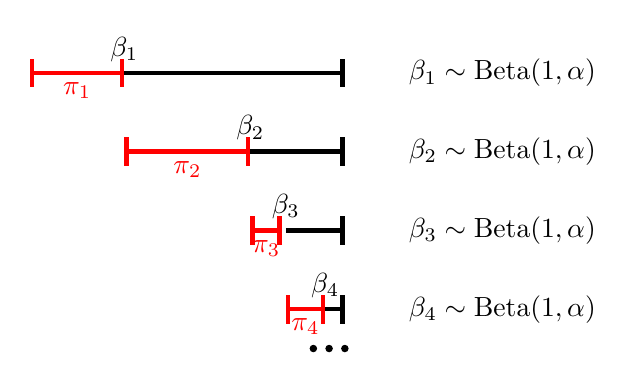
\begin{tikzpicture}
\draw [ultra thick,red,|-|] (0,0) -- (1.2,0);
\draw [ultra thick,-|] (1.2,0) node [above] {$\beta_1$} -- (4,0);
\draw [ultra thick,red,|-|] (1.2,-1) -- (2.8,-1);
\draw [ultra thick, -|] (2.8,-1) node [above] {$\beta_2$} -- (4,-1);
\draw [ultra thick,red,|-|] (2.8,-2) -- (3.2,-2);
\draw [ultra thick, -|] (3.25,-2) node [above] {$\beta_3$} -- (4,-2);
\draw [ultra thick,red,|-|] (3.25,-3) -- (3.75,-3);
\draw [ultra thick, -|] (3.75,-3) node [above] {$\beta_4$} -- (4,-3);
\draw [fill] (3.6,-3.5) circle [radius=0.04];
\draw [fill] (3.8,-3.5) circle [radius=0.04];
\draw [fill] (4.0,-3.5) circle [radius=0.04];
\node at (0.6,0)[below,red]{$\pi_1$};
\node at (2,-1)[below,red]{$\pi_2$};
\node at (3,-2)[below,red]{$\pi_3$};
\node at (3.5,-3)[below,red]{$\pi_4$};
\node at (6,0) {$\beta_1 \sim \Beta(1,\alpha)$};
\node at (6,-1) {$\beta_2 \sim \Beta(1,\alpha)$};
\node at (6,-2) {$\beta_3 \sim \Beta(1,\alpha)$};
\node at (6,-3) {$\beta_4 \sim \Beta(1,\alpha)$};
\end{tikzpicture}
\caption{Stick-breaking construction of $\bs \pi$.}
\label{fig:stick}
\end{figure}

Next, generate a sequence of samples $\theta^{(k)} \sim H$ and let
\begin{equation}
G = \sum_{k=1}^\infty \pi_k \delta_{\theta^{(k)}}
\end{equation}

Sethuraman \cite{sethuraman94} proved that $G \sim \DP(\alpha,H)$ under very general conditions (thereby also giving a more straightforward and general proof of the existence of Dirichlet processes than seen before).
The stick-breaking construction shows in a very straightforward way that samples from a Dirichlet distribution are discrete measures.

\subsubsection*{\normalfont \small \bfseries Clustering property of the Dirichlet process}
\label{sect:clust}
In this section, we will explore the clustering property of Dirichlet processes.

Given a set of samples $\theta^{(1)},\dots,\theta^{(N)}$ generated via the Blackwell-MacQueen urn scheme, we used equation (\ref{eqn:dpprobsame}) to argue that there is a positive probability several samples take on the same value.
Since we have repeated values, let us denote the distinct values by $\bar \theta_1, \dots, \bar \theta_K$, where $K \leq N$.
We may think of these disctinct values as different clusters.

The clustering induced by the DP exhibits a so-called rich-gets-richer behaviour, in that large clusters grow faster than small clusters.
To see that, consider again equation (\ref{eqn:dpprobsame}) and note that it implies that
\begin{equation}
Pr(\theta^{(N+1)} = \bar \theta_k) \propto N_k = \sum_{i=1}^N \mathbbm{1}\{\theta^{(i)} = \bar \theta_k\}.
\end{equation}
Thus, the larger the cluster size $N_k$, the greater the probability that a new sample joins cluster $k$.

\subsubsection*{\normalfont \small \bfseries The Chinese-Restaurant Process}
\label{sect:crp}

\begin{figure}
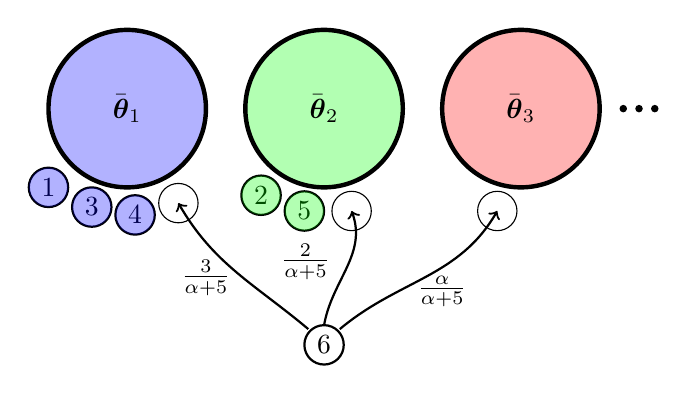
\begin{tikzpicture}
\draw [fill=blue, opacity=0.3] (1,0) circle [radius=1];
\draw [ultra thick] (1,0) node {$\bar{\bs \theta}_1$} circle [radius=1];
\draw [fill=green, opacity=0.3] (3.5,0) circle [radius=1];
\draw [ultra thick] (3.5,0) node {$\bar{\bs \theta}_2$} circle [radius=1];
\draw [fill=red, opacity=0.3] (6,0) circle [radius=1];
\draw [ultra thick] (6,0) node {$\bar{\bs \theta}_3$} circle [radius=1];
\draw [fill] (7.3,0) circle [radius=0.04];
\draw [fill] (7.5,0) circle [radius=0.04];
\draw [fill] (7.7,0) circle [radius=0.04];
\draw [thick] (0,-1) node {$1$} circle [radius=0.25];
\draw [thick] (0.55,-1.25) node {$3$} circle [radius=0.25];
\draw [thick] (1.1,-1.35) node {$4$} circle [radius=0.25];
\draw [thick] (2.7,-1.1) node {$2$} circle [radius=0.25];
\draw [thick] (3.25,-1.3) node {$5$} circle [radius=0.25];
\draw [thick] (3.5,-3) node {$6$} circle [radius=0.25];
\draw [fill=blue,opacity=0.3] (0,-1) circle [radius=0.25];
\draw [fill=blue,opacity=0.3] (0.55,-1.25) circle [radius=0.25];
\draw [fill=blue,opacity=0.3] (1.1,-1.35) circle [radius=0.25];
\draw [fill=green,opacity=0.3] (2.7,-1.1) circle [radius=0.25];
\draw [fill=green,opacity=0.3] (3.25,-1.3) circle [radius=0.25];
\draw [thick,->] (3.3,-2.8) [out=140,in=300] to (1.65,-1.2);
\draw [thin] (1.65,-1.2) circle [radius=0.25];
\draw [thick,->] (3.5,-2.75) [out=80,in=290] to (3.85,-1.3);
\draw [thin] (3.85,-1.3) circle [radius=0.25];
\draw [thick,->] (3.7,-2.8) [out=40,in=240] to (5.7,-1.3);
\draw [thin] (5.7,-1.3) circle [radius=0.25];
\node at (2,-1.8) [below] {$\frac{3}{\alpha+5}$};
\node at (3.7,-1.6) [below left] {$\frac{2}{\alpha+5}$};
\node at (5,-2) [below] {$\frac{\alpha}{\alpha+5}$};
\end{tikzpicture}
\caption{The Chinese restaurant process.
5 customers are currently seated across 2 tables ($K=2$).
The 6th customer is waiting to be seated.
The quantities on the arrows are the probabilities with which customer 6 will be seated at the corresponding table.
Currently, the induced partition over the integers $\{1,2,3,4,5\}$ is $\{\{1,3,4\},\{2,5\}\}$.}
\label{fig:crp}
\end{figure}

We now show that a DP induces a distribution over partitions of integers known as the \emph{Chinese restaurant process} (CRP).
The CRP teases out the clustering property from the DP, just like the stick-breaking construction teased out the discreteness-property.

Consider again our samples $\theta^{(1)},\dots,\theta^{(N)}$ and its unique values $\bar \theta_1,\dots,\bar \theta_K$.
This sample induces a partitioning of the set of integers $[N] = {1,\dots,N}$ into $K$ clusters such that $i$ is in cluster $k$ if $\theta^{(i)} = \bar \theta_k$.
Since our values $\theta^{(i)}$ are randomly, the induced partitioning is also random and its distribution is known as the Chinese restaurant process.

The name is due to a metaphor in which we have a Chinese restaurant with an infinite number of tables and each table can seat an infinite number of customers.
At first, the restaurant is empty and the first customer is seated at the first table. 
The $(i+1)$th customer enters the restaurant is either seated at an already occupied table $k$ or at a new (empty) table $K+1$, with the following probabilities
\begin{equation}
\label{eqn:crp}
\begin{split}
\mbox{Pr($i$ sits at table $k$)} &= \frac{N_k}{i+\alpha}\\
\mbox{Pr($i$ sits at a new table $K+1$)} &= \frac{\alpha}{i+\alpha}
\end{split}
\end{equation}
where $N_k$ is the current number of people sitting at table $k$.
In the metaphor, integers correspond to customers and tables correspond to clusters. 
After the $N$th customer is seated, the tables define a partition of $[N]$ and its distribution is the same as the one induced by the DP.

Note that the probability of opening up a new table, i.e. of creating a new cluster is proportional to the concentration parameter $\alpha$.
If $\alpha$ is large, we should expect to see many distinct values $\bar \theta_1,\dots,\bar \theta_K$.
In other words, $K$ increases with $\alpha$ on average and it is possible to show that the number of occupied tables, $K$, approaches $\alpha \log(N)$ as $N \rightarrow \infty$ (in probability).

It is possible to start with CRP and get back to the Blackwell-MacQueen urn scheme (and thus the Dirichlet process). 
For each table $k$, we draw a value $\bar \theta_k$ from the base distribution, $\bar \theta_k \sim H$.
We then set all samples whose index is in cluster $k$ (i.e. who ``sit" at table $k$) equal to that value
\begin{equation}
\theta^{(i)} = \bar \theta_{z_i}
\end{equation}
where $z_i$ is the table at which customer $i$ is sitting at.

We will return to the Chinese restaurant process in the next section when we discuss Dirichlet mixtures as it builds the basis for our inference method.

\section{The Dirichlet Process Mixture}
\label{sect:DPM}
So far, the discussion has been about the properties of the Dirichlet process as a stochastic object.
In this section, we show how Dirichlet processes can be used for clustering and to model data via \emph{Dirchlet process mixtures (DPM)}.
We first describe the model in general terms.
Next we explain how to fit the parameters of the model via Gibbs sampling and give a brief overview of alternative inference methods.
Following this, we go in detail through our C++ implementation of the DPM with a Normal Inverse Wishart conjugate prior and give a brief demonstration on some test data.

\subsection{Density Estimation and Clustering using Dirichlet Processes}
Suppose we have a dataset $S = \{x^{(i)}\}_{i=1}^N$ that are independently drawn from some unknown distribution and suppose we would like to estimate the density of this distribution.
In the Bayesian nonparametric literature, the standard approach is to put a nonparametric prior distribution over the space of distributions.
The aim is to have a very flexible model (since we are not limiting ourselves to some parametric family but instead considering all distributions) while also avoiding overfitting (by using Bayesian inference).
The Dirichlet process provides a good choice for our prior as it has broad cover over the space of distributions while also being mathematically convenient (through conjugacy).
However, we saw that draws from a DP are discrete distributions and therefore not particularly useful as a direct model for real data.
To get around this problem, we convolve the DP with a smooth distribution to create a nonparametric density for our data.

Let $G \sim \DP(\alpha,H)$ and let $f(x|\,\theta)$ be a parametric family of smooth densities with parameters $\theta$. 
For example, we may use $f(x|\,\theta) = \mathcal{N}(x|\,\mu,\Sigma)$ in which case $\theta = (\mu,\Sigma)$.
The density of x is then modelled as 
\begin{equation}
p(x) = \int f(x|\,\theta)\, G(\theta)d\theta.
\end{equation}

This model is a mixture of distributions in which $G$ is the mixing distribution over $\theta$ and $F(\theta)$ are the base distributions with density functions $f(x|\,\theta)$.
More precisely, we model out data set $S$ using a set of \emph{latent parameters} $\{\theta^{(i)}\}$.
The parameters are drawn independently from $G$ and the distribution of each $x^{(i)}$ is given by $F(\theta^{(i)})$:
\begin{equation}
\label{eqn:dpm}
\begin{split}
G &\sim \DP(\alpha,H)\\
\theta^{(i)} |\,G &\sim G\\
x^{(i)} |\,\theta^{(i)} &\sim F(\theta^{(i)})
\end{split}
\end{equation}
We assume that, given the $\theta^{(i)}$, the observations $x^{(i)}$ are independent of each other and of $G$.

We already saw that multiple $\theta^{(i)}$ can take on the same value (due to the discreteness of $G$).
Thus, as well as density estimation, we can also use this model for clustering where observations $x^{(i)}$ whose parameter $\theta^{(i)}$ take on the same value belong to the same cluster.

To make the connection to mixture models more explicit, we introduce a latent categorical variable $z^{(i)} \in \{1,2,\dots\}$ that tells us the cluster assignment for each observation $x^{(i)}$.
The DPM model can then be expressed in the following way:
\begin{equation}
\begin{split}
x^{(i)} |\,z^{(i)},\{\bar \theta_1,\bar \theta_2,\dots\} &\sim F(\bar \theta_{z^{(i)}})\\
z^{(i)} |\,\{\pi_1,\pi_2,\dots\} &\sim \Cat(\pi_1,\pi_2,\dots)\\
\bar \theta_1,\bar \theta_2,\dots &\sim H\\
\pi_1,\pi_2,\dots &\sim \GEM(\alpha)
\end{split}
\end{equation}
so that
\begin{equation}
\label{eqn:dpmmixture}
p(x) = \sum_{k=1}^\infty \pi_k f(x|\,\bar \theta_k)
\end{equation}

In this formulation we see very clearly that Dirichlet process mixtures can be viewed as (countably) infinite mixture models.
However, in any finite data set we can observe at most $K = N$ of the mixture components. In practice, $K<<N$ and as we mentioned earlier, $K$ tends to grow logarithmically with the sample size $N$.

The advantage over using a finite mixture model is that we do not need to specify the number of components $K$, but instead infer it from the data.
However, note that an underlying assumption of the DPM is that the true number of clusters is infinite and thus, the larger our dataset the more clusters we will observe.
For many applications, this assumption is realistic.
But, if we know that the number of clusters in the underlying population is finite, the DPM is a misspecified model. In this case, using a finite mixture model along with a model selection tool is a more appropriate approach.

\subsection{Inference in Dirichlet Process mixtures}
The most popular approaches to inference in Dirichlet process mixture models are based on Markov chain Monte Carlo (MCMC) methods.
The 2000 paper by Radford Neal \cite{neal2000} provides an excellent review of inference methods based on Gibbs sampling using the Chinese restaurant process representation of Dirichlet processes.
In particular, ``algorithm 8" in his paper is still considered to be one of the best MCMC based inference methods for handling non-conjugate priors.
Since then, there have been proposals for better MCMC inference algorithm such as blocked Gibbs sampling based the stick-breaking representation \cite{ishwaran2001}, Metropolis-Hastings with larger moves \cite{jain2004} and sequential Monte Carlo \cite{fearnhead2004}.

Besides MCMC based algorithms, there have also other approaches to inference in DP mixtures.
An algorithm based on expectation propagation was derived by \cite{minka2003}.
The first variational Bayes approximation was developed by \cite{blei2006}.

\subsection{A Gibbs Sampler for Dirichlet Process Mixtures}
Although better methods for inference in DPMs have been developed, we will focus on Gibbs sampling.
The reason for this is two-fold.
First, it is generaly considered to be the standard sampler for Dirichlet Process mixtures and very popular due to its simplicity.
Second, it is the inference method used in the current version of our implementation.

\subsubsection*{\normalfont \small \bfseries Gibbs Sampling}
Recall that a Gibbs sampler simulates random draws $\bs \Phi = (\Phi_1,\dots,\Phi_D)$ from some multivariate distribution $Q$ on $\Omega$ (with $\dim\Omega = D$) by looping over the dimensions $d \in \{1,\dots,D\}$ and sampling $\Phi_d$ from its conditional distribution given the remaining dimensions (the so-called \emph{full conditional} distribution of $\Phi_d$).
When sampling $\Phi_d$ from its full conditional $Q(\Phi_d|\,\bs\Phi_{-d} = \bs \phi_{-d})$, the Gibbs sampler always conditions on the most recently generated values of $\bs \Phi_{-d}$.
\footnote{Recall that we used the $``-d"$ subscript to denote ``all except $d$" so that $\bs \phi_{-d}$ is a short-hand for $(\phi_1,\dots,\phi_{d-1},\phi_{d+1},\dots,\phi_{D})$.}
More explicitly, in the $j$th iteration of the Gibbs sampler, the algorithm samples as follows:
\begin{equation}
\label{eqn:Gibbs}
\begin{split}
\Phi_1^{(j)} &\sim Q(\Phi_1|\,\Phi_2 = \phi_2^{(j-1}),\dots,\Phi_D = \phi_D^{(j-1)})\\
&\vdots\\
\Phi_d^{(j)} &\sim Q(\Phi_d|\,\Phi_1 = \phi_1^{(j)},\dots,\Phi_{d-1}=\phi_{d-1}^{(j)},\\
&\qquad\qquad \Phi_{d+1}=\phi_{d+1}^{(j-1)},\dots,\Phi_D=\phi_D^{(j-1)})\\
&\vdots\\
\Phi_D^{(j)} &\sim Q(\Phi_D|\,\Phi_1=\phi_1^{(j)},\dots,\Phi_{D-1}=\phi_{D-1}^{(j)})
\end{split}
\end{equation}
In practice, it is often more efficient to randomly permute the dimensions at the start of each iteration, so that the components are sampled in a random order.

\subsubsection*{\normalfont \small \bfseries A na{\"i}ve Gibbs sampler}
Recall that in the DPM, observations are assumed to be generated according to (\ref{eqn:dpm}) and that two sample $x^{(i)}$ and $x^{(j)}$ are in the same cluster if $\theta^{(i)}=\theta^{(j)}$.
While the conditional joint distribution of $(\theta^{(1)},\dots,\theta^{(N)})$ given the data is complicated, the derivation of the full conditional $p(\theta^{(i)}|\,\bs\theta^{(-i)},X)$, where $X=\{x^{(1)},\dots,x^{(N)}\}$, is relatively straight forward.
\footnote{Note that, in accordance with the general description on Gibbs sampling above, we view the variables $\theta^{(1)},\dots,\theta^{(N)}$ as $N$ coordinate variables.}
From the Blackwell-MacQueen urn scheme (equation \ref{eqn:dppostpred}), we can derive the following conditional distribution
\begin{equation}
\label{eqn:dpmpostpred}
p(\theta^{(i)}|\,\bs\theta^{(-i)}) = \frac{\alpha H(\theta^{(i)})}{\alpha+N-1} +\frac{\sum_{j\neq i}\delta_{\theta^{(j)}}(\theta^{(i)})}{\alpha+N-1}
\end{equation}
To see why, imagine that observation $I$ is the last of the $N$ observations.
We are allowed to do so because we assumed that the $\theta^{(i)}$ are conditionally independent given $G$ and therefore satisfy the condition of \emph{exchangeability}, meaning that any order of a finite number of samples is equally likely.

Finally, we also need to condition on the observed data.
For that, we use the assumption that, for $j\neq i$, $\theta^{(i)}$ is conditionally independent of observation $x^{(j)}$ given $\theta^{(j)}$.
This means that $p(\theta^{(i)}|\,\bs\theta^{(-i)},X) = p(\theta^{(i)}|\,\bs\theta^{(-i)},x^{(i)})$.
To compute that last quantity we treat $p(\theta^{(i)}|\,\bs\theta^{(-i)})$ as a prior for $\theta^{(i)}$ and compute its posterior under the single observation $x^{(i)}$ using Bayes' rule:
\begin{equation}
\label{eqn:dpmgibbs1}
p(\theta^{(i)}|\,\bs\theta^{(-i)},x^{(i)}) = \frac{p(\theta^{(i)}|\,\bs\theta^{(-i)})f(x^{(i)}|\,\theta^{(i)})}{\int_\Omega p(\theta|\,\bs\theta^{(-i)})f(x^{(i)}|\,\theta) d\theta}\\
\end{equation}
\begin{equation*}
=\frac{\alpha H(\theta^{(i)})f(x^{(i)}|\,\theta^{(i)}) + \sum_{j\neq i}f(x^{(i)}|\,\theta^{(i)})\delta_{\theta^{(j)}}(\theta^{(i)})}{\left(\alpha\int_\Omega H(\theta)f(x^{(i)}|\,\theta)d\theta+\sum_{j \neq i}f(x^{(i)}|\,\theta^{(j)})\right)}
\end{equation*}
In order for this algorithm to be feasable, we need to be able to compute the integral in equation (\ref{eqn:dpmgibbs1}).
This is generally the case when $H$ is conjugate to $f$.

The resulting inference method is summarized in algorithm \ref{alg:naive}.
\begin{algorithm}
\caption{Na{\"i}ve Gibbs sampler for DP mixtures}
\label{alg:naive}
\begin{algorithmic}[1]
\State Initialize $\theta^{(1)},\dots,\theta^{(N)}$
\State Set the total number of Gibbs iterations $L$
\For{$j=1,\dots,L$}
\For{$i=1,\dots,N$ in random order}
\State Sample $\theta^{(i)}|\,\bs\theta^{(-i)},x^{(i)}$ according to (\ref{eqn:dpmgibbs1})
\EndFor
\EndFor
\State\Return $\{\theta^{(1)},\dots,\theta^{(N)}\}$
\end{algorithmic}
\end{algorithm}

The algorithm was developed by \cite{escobar1994} and used in \cite{escobar1995}.
It is a valid sampler corresponding to ``algorithm 1" in \cite{neal2000}.
However, convergence to the true posterior distribution is generally very slow (we say it has slow mixing behaviour).
The reason is that often, multiple samples $x$ will be associated with the same parameter value $\theta$ (which is why we are able to use the model for clustering in the first place).
However, the algorithm is unable to change the parameter value for more than one $x$ simultaneously. 
So in order for the algorithm to change the parameter value for all $x$ within a cluster, it has to do so individually for each observation, thereby passing through a low-probability intermediate state in which the cluster is split.

\subsubsection*{\normalfont \small \bfseries An improved Gibbs Sampler}
We can improve our algorithm by splitting up inference for the cluster assignments and inference for the cluster parameters.
To do this, we again introduce our cluster assignment variable $z^{(i)}$ defined such that $z^{(i)}=k$ if and only if $x^{(i)}$ is in cluster $k$.
We also shift focus to the distinct cluster parameters $\bar \theta_1,\dots,\bar \theta_K$ present in our data. 

A Gibbs iteration now consists of two distinct loops.
First, for each $i$, we remove $x^{(i)}$ from its current cluster and sample a new cluster assignment $z^{(i)}$ from the full conditional.
Next, we sample a parameter $\bar \theta_k$ from the posterior for each currently present cluster $k$.

We can derive the full conditionals for the $z^{(i)}$ from equation (\ref{eqn:dpmgibbs1}) in the following way (where we use $\overline {\bs \theta}_{-k}$ to denote the collection of all currently present cluster parameters, $\bs{\overline\theta}=\{\overline \theta_1,\dots,\overline \theta_K\}$):
\begin{equation}
\begin{split}
&\Pr(z^{(i)}=k|\,\bs z^{(-i)},\overline {\bs \theta},x^{(i)}) = \Pr(\theta^{(i)} \in \{\bar \theta_k\}|\,\bs z^{(-i)},\overline {\bs \theta},x^{(i)})\\
&= \int_{\{\bar \theta_k\}} p(\theta|\,\bs\theta^{(-i)},x^{(i)}) d\theta\\
%&= \frac{1}{B}\int_{\{\bar \theta_k\}}\left(\alpha H(\theta)f(x^{(i)}|\,\theta)d\theta + \sum_{j\neq i}f(x^{(i)}|\,\theta)\delta_{\theta^{(j)}}(\theta)\right)d\theta\\
&= B \left[\alpha\int_{\{\bar \theta_k\}} H(\theta)f(x^{(i)}|\,\theta)d\theta + \sum_{j\neq i}\int_{\{\bar \theta_k\}}f(x^{(i)}|\,\theta)\delta_{\theta^{(j)}}(\theta)d\theta\right]
\end{split}
\end{equation}
where we used $B$ to denote the normalization constant (i.e. the inverse of the denominator in equation (\ref{eqn:dpmgibbs1})).
Note that, if $H$ and $F$ are smooth distributions (i.e. do not contain point-masses) then integrating them over a single point results in zero.
Thus, we are left with
\begin{equation}
\label{eqn:phi_k}
\begin{split}
\Pr(z^{(i)}=k|\,\bs z^{(-i)},\overline {\bs \theta},x^{(i)}) &= B f(x^{(i)}|\,\bar\theta_k)\sum_{j\neq i}\mathbbm{1}\left\{\theta^{(j)} = \bar \theta_k\right\} \\
&= B f(x^{(i)}|\,\bar\theta_k)N_k^{\,(-i)}\\
&= \phi_k
\end{split}
\end{equation}
where $N_k^{\,(-i)}$ is the current size of cluster $k$ without counting sample $x^{(i)}$.

Of course, it is also possible that $x^{(i)}$ is in none of the current clusters.
We may represent this by letting $z^{(i)} = K+1$, where $K$ is the current number of clusters (without counting sample $x^{(i)}$).
The conditional probability is given by 
\begin{equation}
\begin{split}
&\Pr(z^{(i)}=K+1|\,\bs z^{(-i)},\overline {\bs \theta},x^{(i)}) = \Pr(\theta^{(i)} \in \Omega/\bs{\overline \theta}|\,\bs z^{(-i)},\overline {\bs \theta},x^{(i)})\\
%&= \int_{\Omega/\overline{\bs\theta}} p(\theta|\,\bs\theta^{(-i)},x^{(i)}) d\theta\\
&= B\left[\alpha\int_{\Omega/\overline{\bs\theta}} H(\theta)f(x^{(i)}|\,\theta)d\theta + \sum_{j\neq i}\int_{\Omega/\overline{\bs\theta}}f(x^{(i)}|\,\theta)\delta_{\theta^{(j)}}(\theta)d\theta\right]
\end{split}
\end{equation}
This time, the integral over the delta function terms vanishes since $\theta^{(j)}\in \overline{\bs\theta}$ for all $j\neq i$ and we are excluding those points from the domain of integration.
Moreover, the integrand in the first term is continuous and so, taking its integral over $\Omega/\overline{\bs\theta}$ yields the same result as taking its integral over the entire space $\Omega$ since we are only excluding countably many points.
Thus
\begin{equation}
\label{eqn:phi_K+1}
\begin{split}
\Pr(z^{(i)}=K+1|\,\bs z^{(-i)},\overline {\bs \theta},x^{(i)}) &= B\, \alpha \int_\Omega H(\theta)f(x^{(i)}|\,\theta)d\theta\\
&= \phi_{K+1}
\end{split}
\end{equation}

\begin{algorithm}
\caption{Gibbs sampling inference for DP mixtures}
\begin{algorithmic}[1]
\State Set the initial number of occupied clusters $K$
\State Initialize $\bar \theta_1,\dots, \bar \theta_K$ and $z^{(1)},\dots,z^{(N)}$
\State Set the total number of Gibbs iterations $L$
\For {$j=1,\dots,L$}
\For {$i = 1,\dots,N$ in random order}
%\State Remove $i$ from its current cluster: 
\State Set $N_{z^{(i)}}=N_{z^{(i)}}-1$
\If {$N_{z^{(i)}}=0$}
\State Remove cluster $k$: Delete $\bar \theta_k$
\State Set $K = K - 1$
\State Rearrange indeces $k$ such that clusters 
\State \quad $k=1,\dots,K$ are non-empty clusters
\EndIf
\State Sample $z^{(i)}$ according to (\ref{eqn:samplez})%\sim \Cat(\phi_1,\dots,\phi_{K+1})$ according
%\State \qquad to equations (\ref{eqn:phi_k}) and (\ref{eqn:phi_K+1})
\If {$z^{(i)}=K+1$}
\State Sample $\bar \theta_{K+1}$ according to (\ref{eqn:newcluster})
\State Set $K=K+1$
\EndIf
\EndFor
\For {$k=1,\dots,K$}
\State Sample $\bar \theta_k$ according to (\ref{eqn:sampletheta})
\EndFor
\EndFor
\State\Return $\{z^{(1)},\dots,z^{(N)}\}$, \, $\{\bar \theta_1,\dots,\bar\theta_K\}$
\end{algorithmic}
\label{alg:gibbs2}
\end{algorithm}

Having worked out the full conditionals, we can sample 
\begin{equation}
\label{eqn:samplez}
z^{(i)}|\,\bs z^{(-i)},\overline {\bs \theta},x^{(i)} \sim \Cat(\phi_1,\dots,\phi_K,\phi_{K+1})
\end{equation}
If $z^{(i)}=K+1$, $x^{(i)}$ is joining an empty cluster and we therefore need to sample a new parameter $\bar \theta_{K+1}$.
The new parameter is sampled from the posterior distribution for $\theta$ based on the prior $H$ and the single observation $x^{(i)}$:
\begin{equation}
\label{eqn:newcluster}
\bar \theta_{K+1}|\,x^{(i)} \sim \frac{H(\theta)f(x^{(i)}|\,\theta)}{\int_\Omega H(\theta')f(x^{(i)}|\,\theta')d\theta'}
\end{equation}
We also need to increment $K$ by 1 in this case.
This completes the first part of the Gibbs sampler.

In the second part of the algorithm, we loop over each currently present cluster $k$ and sample a new parameter $\bar \theta_k$ for that cluster.
The sample is drawn from the posterior distribution of $\theta$ based on the prior $H$ and all data points that are currently in cluster $k$:
\begin{equation}
\label{eqn:sampletheta}
\bar \theta_k |\,\{x^{(i)}:z^{(i)}=k\} \sim \frac{\left(\prod_{i:z^{(i)}=k}f(x^{(i)}|\,\theta)\right)H(\theta)}{\int_\Omega\left(\prod_{i:z^{(i)}=k}f(x^{(i)}|\,\theta')\right)H(\theta')d\theta'}
\end{equation}
Note that we have dealt with the problem that we faced in the na{\"i}ve Gibbs sampler.
We now draw a new parameter value $\bar \theta_k$ for all datapoints in cluster $k$ simultaneously.

In the Chinese restaurant metaphor, the first part of the algorithm corresponds to individually asking each customer $i$ to get up from her current table and join a new table table at random.
The probability for joining table $k$ depends on what ``dish" $\bar \theta_k$ is currently being served at that table. It is also possible for the customer to join a currently empty table, in which case a new dish will be served according to her taste (thinking of $x^{(i)}$ as ``culinary preferences").
Once we have made each customer move, we clean all the tables and serve a new dish at each table (taking into account the preferences of the customers sitting at that table).

We have summarized this inference method in algorithm \ref{alg:gibbs2}.
This is the standard sample for Dirichlet process mixtures.
It is due to \cite{maceachern1994} and corresponds to ``algorithm 2" in Neal's paper \cite{neal2000}.

As was the case for the previous Gibbs sampler, this method is only feasable if we can efficiently compute the integrals in (\ref{eqn:phi_K+1}),(\ref{eqn:newcluster}) and (\ref{eqn:sampletheta}).
This is generally the case if $H$ is the conjugate prior to the likelihood function $f$.

Lastly, we briefly return to the problem of density estimation.
After running our Gibbs sampler, we have estimates for the cluster assignments and the cluster parameters.
Using these, we are able to formulate the posterior predictive distribution for a new sample $x^{(N+1)}$ as follows
\begin{equation}
\label{eqn:dompostpred}
\begin{split}
p(x^{(N+1)}|\,x^{(1)},\dots,x^{(N)}) &= \sum_{k=1}^K \frac{N_k}{\alpha+N}f(x^{(N+1)}|\,\bar\theta_k)\\
&+ \frac{\alpha}{\alpha+N}\int_\Omega f(x^{(N+1)}|\,\theta)H(\theta)d\theta
\end{split}
\end{equation}
Comparing this with the mixture density in (\ref{eqn:dpmmixture}), we can set the mixing coefficients $\pi_1,\dots,\pi_K$ as follows
\begin{equation}
\pi_k = \frac{N_k}{\alpha+N}
\end{equation}
We are only able to find explicit formulas for the clusters that we have estimated to be present in our data set.
The second term in the posterior predictive corresponds to all clusters that are currently empty (of which there are an infinite number).
We can interpret $\int_\Omega f(x^{(N+1)}|\,\theta)H(\theta)d\theta$ as a mixture component representing the possibility that $x^{(N+1)}$ does not belong to any of the other clusters. 

For more details on Gibbs sampling in DP mixtures, see \cite{neal2000,orbanz2014}.


\section{Implementation of the Normal-Inverse-Wishart Dirichlet Process Mixture model}
In this section, we will describe our implementation of the Dirichlet process mixture model.
We assumed that our data lives in $D$-dimensional Euclidean space, $\bs x \in \mathbb{R}^D$, and therefore chose a Gaussian likelihood model with a conjugate prior.

\subsection{Bayesian analysis of the multivariate Gaussian}
Before descibing the details of the implementation, we shall briefly review Bayesian inference for the Gaussian distribution.

Suppose we have a set of $D$-dimensional variables $X^{(1)},\dots,X^{(N)}$ that are independent and identically distributed according to a multivariate Gaussian distribution with mean $\bs\mu \in \mathbb{R}^D$ and covariance matrix $\bs\Sigma \in \mathbb{R}^{D\times D}$. 
The pdf of the Gaussian is given by
\begin{equation}
\mathcal{N}(\bs x|\,\bs\mu,\bs\Sigma) = (2\pi)^{-\frac{1}{2}D}|\bs\Sigma|^{-\frac{1}{2}} \exp \left((\bs\mu-\bs x)^T \bs\Sigma^{-1} (\bs\mu-\bs x) \right).
\end{equation}

If we have a dataset of observations $S = \{\bs x^{(1)},\dots,\bs x^{(N)}\}$ so that $X^{(i)} = \bs x^{(i)}$, we can formulate the likelihood of the data as follows
\begin{equation}
p(S|\,\bs\mu,\bs\Sigma) = \prod_{i=1}^N \mathcal{N}(\bs x^{(i)}|\,\bs \mu,\bs \Sigma).
\end{equation}

For simplicity, we will put a conjugate prior over the parameters $(\bs\mu,\bs\Sigma)$ which, in our case, is the \emph{Normal-inverse-Wishart} (NIW) distribution.
Its density function is defined as follows
\begin{equation}
\begin{split}
\mathcal{NIW}&(\bs\mu,\bs\Sigma|\,\bs m_0,\kappa_0,\bs S_0,\nu_0) = Z_{NIW}|\bs\Sigma|^{-\frac{\nu_0+D+2}{2}} \,\times\\
& \exp\left(-\frac{\kappa_0}{2}(\bs\mu-\bs m_0)^T\bs\Sigma^{-1}(\bs\mu-\bs m_0) -\frac{1}{2}\Tr(\bs\Sigma^{-1}\bs S_0) \right)
\end{split}
\end{equation}

where $Z_{NIW}$ is the normalization constant defined by
\begin{equation}
\frac{1}{Z_{NIW}} = 2^{\frac{\nu_0 D}{2}}\left(\frac{2\pi}{\kappa_0}\right)^{\frac{D}{2}}|\bs S_0|^{-\frac{\nu_0}{2}}\Gamma_D \left(\frac{\nu_0}{2}\right)
\end{equation}

and $\Gamma_D$ is the multivariate Gamma function defined as
\begin{equation}
\Gamma_D(t) = \pi^{\frac{D(D-1)}{4}} \prod_{j=1}^D \Gamma\left(t + \frac{1-j}{2}\right)
\end{equation}

We can interpret the hyper-parameters $\lambda = (\bs m_0,\kappa_0,\bs S_0,\nu_0)$ as follows:
$\bs m_0 \in \mathbb{R}^D$ is our prior belief for $\bs \mu$ and $\kappa_0 > 0$ is the strength of that belief.
The so-called scale matrix $\bs S_0$ is a positive definite $D\times D$ matrix and represents our prior belief for $\bs \Sigma$ (it is proportional to the prior mean of $\bs\Sigma$).
The final hyper-parameter $\nu_0$ is called the ``degrees of freedom". It must satisfy $\nu_0 \geq D$ measures the strength of our belief in the prior for $\Sigma$.

The posterior for our parameters $(\bs\mu,\bs\Sigma)$ is given by
\begin{equation}
\begin{split}
&p(\bs\mu,\bs\Sigma|\,S) =\\
&\frac{\mathcal{NIW}(\bs\mu,\bs\Sigma|\,\bs m_0,\kappa_0,\bs S_0,\nu_0)\prod_{i=1}^N \mathcal{N}(\bs x^{(i)}|\,\bs \mu,\bs \Sigma)}{\iint\mathcal{NIW}(\bs\mu,\bs\Sigma|\,\bs m_0,\kappa_0,\bs S_0,\nu_0)\prod_{i=1}^N \mathcal{N}(\bs x^{(i)}|\,\bs \mu,\bs \Sigma)d(\bs\mu,\bs\Sigma)}\\
&= \mathcal{NIW}(\bs\mu,\bs\Sigma|\,\bs m_n,\kappa_N,\bs S_N,\nu_N)
\end{split}
\end{equation}


%\section{Extensions and Further Work}

\section*{Acknowledgements}
Here I acknowledge the assistance of my supervisor, my industrial sponsor,
and the effects of caffeine on my ability to produce this report on time.

%% The Appendices part is started with the command \appendix;
%% appendix sections are then done as normal sections
\appendix

%% References
%%
%% Following citation commands can be used in the body text:
%% Usage of \cite is as follows:
%%   \cite{key}         ==>>  [#]
%%   \cite[chap. 2]{key} ==>> [#, chap. 2]
%%

%% References with bibTeX database:
\section*{Bibliography}
%\bibliographystyle{elsarticle-num}
\bibliographystyle{apa}
\bibliography{references.bib}

%% Authors are advised to submit their bibtex database files. They are
%% requested to list a bibtex style file in the manuscript if they do
%% not want to use elsarticle-num.bst.

%% References without bibTeX database:

% \begin{thebibliography}{00}

%% \bibitem must have the following form:
%%   \bibitem{key}...
%%

% \bibitem{}

% \end{thebibliography}


\end{document}

%%
%% End of file `mini.tex'.